\documentclass[tikz,border=9pt]{standalone}
\usepackage{amsmath}
\usetikzlibrary{arrows.meta,calc,positioning}
\definecolor{starkblue}{HTML}{0072B2}
\definecolor{starkgreen}{HTML}{009E73}
\definecolor{starkgold}{HTML}{E69F00}
\definecolor{starkpurple}{HTML}{CC79A7}
\definecolor{starkred}{HTML}{D55E00}
\begin{document}
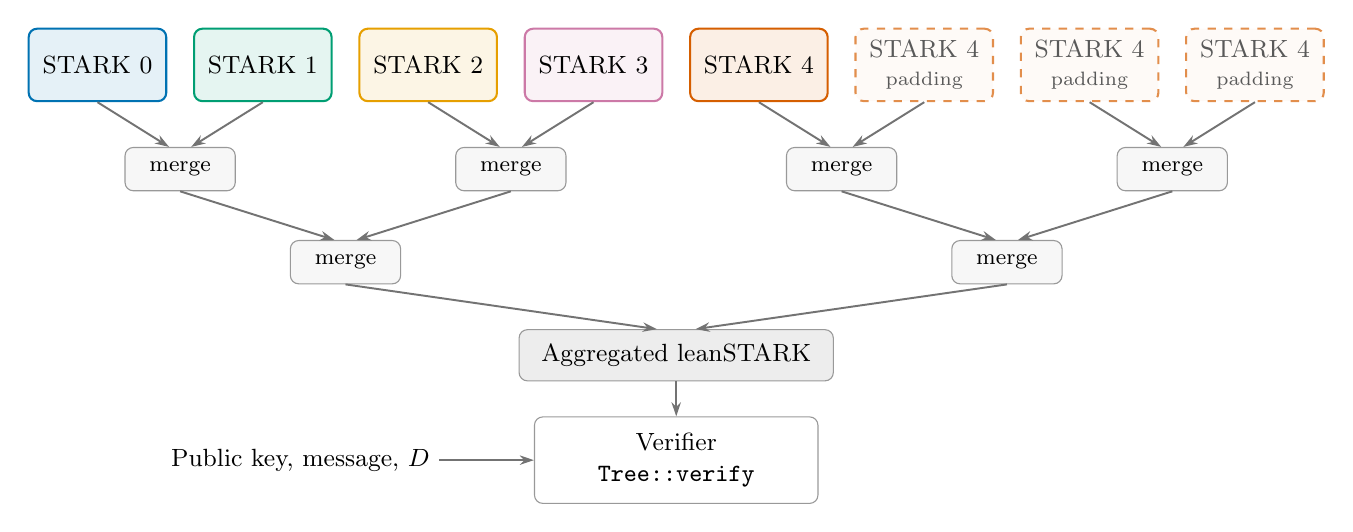
\begin{tikzpicture}[font=\fontsize{9}{11}\selectfont,
 arrow/.style={-{Stealth[length=1.8mm,width=1.2mm]},line width=.7pt,draw=black!55},
 leaf/.style={rounded corners=3pt,draw,line width=.75pt,
   inner xsep=5pt,inner ysep=4pt,
   minimum width=1.65cm,minimum height=.92cm,align=center},
 merge/.style={rounded corners=3pt,draw=black!40,fill=black!3,
   font=\fontsize{8.5}{10.5}\selectfont,inner xsep=8pt,inner ysep=4pt,
   minimum width=1.4cm,minimum height=.55cm,align=center}]

\foreach \p/\col in {0/starkblue,1/starkgreen,2/starkgold,3/starkpurple,4/starkred} {
 \pgfmathsetmacro{\xp}{.8+2.1*\p}
 \node[leaf,draw=\col,fill=\col!10] (L\p) at (\xp,0) {STARK \p};
}
\foreach \p in {5,6,7} {
 \pgfmathsetmacro{\xp}{.8+2.1*\p}
 \node[leaf,draw=starkred!70,dashed,fill=starkred!3,text=black!65]
   (L\p) at (\xp,0) {STARK 4\\[-1pt]\fontsize{7.5}{9}\selectfont padding};
}

\foreach \p/\a/\b in {0/0/1,1/2/3,2/4/5,3/6/7} {
 \node[merge] (M\p) at ($(L\a.south)!.5!(L\b.south)+(0,-.85)$) {merge};
 \draw[arrow] (L\a.south) -- ([xshift=-4pt]M\p.north);
 \draw[arrow] (L\b.south) -- ([xshift=4pt]M\p.north);
}
\foreach \p/\a/\b in {0/0/1,1/2/3} {
 \node[merge] (N\p) at ($(M\a.south)!.5!(M\b.south)+(0,-.90)$) {merge};
 \draw[arrow] (M\a.south) -- ([xshift=-4pt]N\p.north);
 \draw[arrow] (M\b.south) -- ([xshift=4pt]N\p.north);
}
\node[merge,font=\fontsize{9}{11}\selectfont,fill=black!7,
  minimum width=3.6cm,minimum height=.65cm]
  (Root) at ($(N0.south)!.5!(N1.south)+(0,-.90)$) {Aggregated leanSTARK};
\draw[arrow] (N0.south) -- ([xshift=-7pt]Root.north);
\draw[arrow] (N1.south) -- ([xshift=7pt]Root.north);

\node[draw=black!40,rounded corners=3pt,align=center,inner xsep=8pt,inner ysep=6pt,
  minimum width=3.6cm,minimum height=.92cm] (Verifier) at ($(Root.south)+(0,-1.0)$)
  {Verifier\\\texttt{Tree::verify}};
\draw[arrow] (Root.south) -- (Verifier.north);
\node[anchor=east,align=center] (Public) at ($(Verifier.west)+(-1.2,0)$)
  {Public key, message, $D$};
\draw[arrow] (Public.east) -- (Verifier.west);

\end{tikzpicture}
\end{document}
